\graphicspath{{images/program}}

\section{Programm}

% In diesem Kapitel wird das Programm beschrieben, welches die Fotobox steuert.
% Zuerst grober aufbau mitteld diagramm und beschreibung einzelner komponenten. dann in späteren kapiteln genauere beschreibung.

Die Fotobox Software ist aus mehreren einzelnen Softwarekomponenten aufgebaut,
unter anderem dem Windows Programm, welches dafür zuständig ist, die Kamera
und den Drucker zu steuern, das live Bild der Kamera auf dem Laptop anzuzeigen,
und die aufgenommenen Bilder zu verarbeiten. Dem Webserver, welcher dazu dient,
die Bilder zu organisieren, und die Website anzuzeigen, über welche die Fotobox
konfiguriert werden kann, und man die Bilder herunterladen kann.

\subsection{}
\begin{figure}[H]
    \centering
    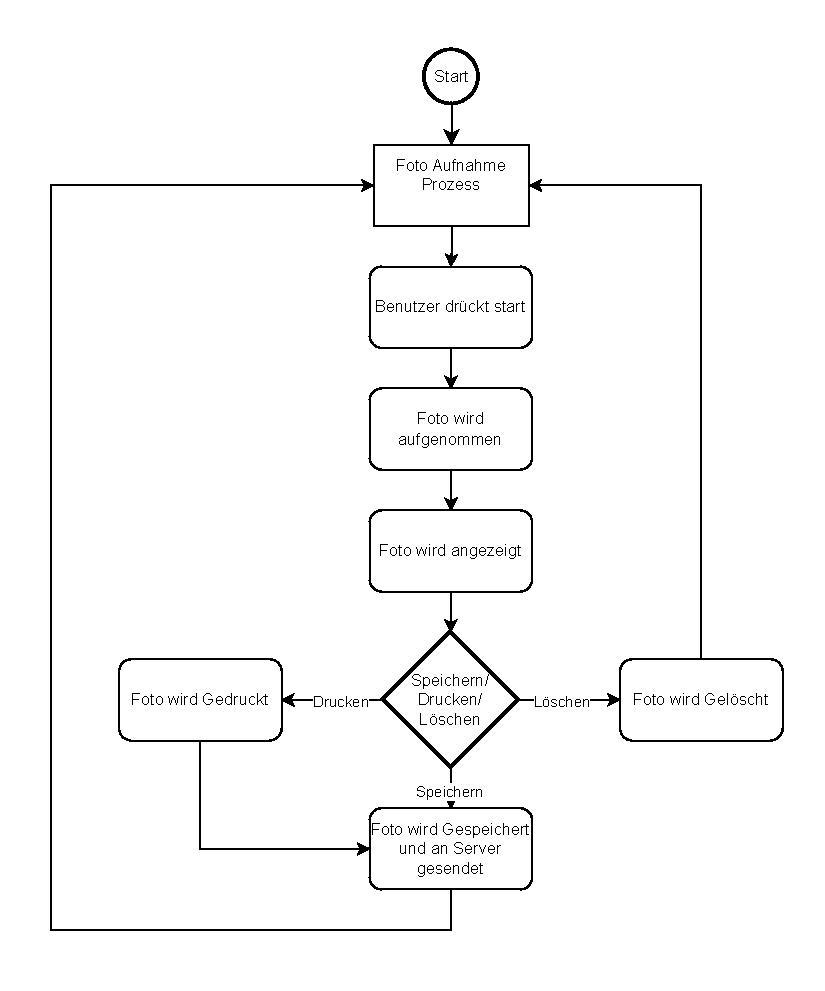
\includegraphics[width=1\textwidth]{Ablauf_Foto_Aufnehmen.drawio.pdf}
    \caption{Ablaufdiagramm der Fotoaufnahme.}
    \label{fig:Ablauf_Foto_Aufnehmen}
\end{figure}